% move all configuration stuff into one file so we can focus on the content
\documentclass[aspectratio=169,hyperref={pdfpagelabels=false,colorlinks=true,linkcolor=white,urlcolor=lightblue},xcolor={table},t]{beamer}

%%%%%%%%%%%%%%%%%%%%%%%%%%%%%%%%%%%%%%%%%%%%%%%%%%%%%%%%%%%%%%%%%%%%%%%%%%%%%%%%%%
%%%%%%%%%%%%%%%%%%%%%%%%%%%%%%%%%%%%%%%%%%%%%%%%%%%%%%%%%%%%%%%%%%%%%%%%%%%%%%%%%%
% packages
\usepackage{pict2e}
\usepackage{epic}
\usepackage{amsmath,amsfonts,amssymb}
\usepackage{units}
\usepackage{fancybox}
\usepackage[absolute,overlay]{textpos} 
%\usepackage[table]{xcolor}
\usepackage{animate}
\usepackage{gensymb}
%\usepackage{graphicx}
%\usepackage{longtable}
\usepackage{multirow}
\usepackage{silence}
\usepackage{tikz}
\usepackage[backend=bibtex,style=ieee]{biblatex}
\AtEveryCitekey{\iffootnote{\tiny}{}}
%\addbibresource{include/references}



% fontsize
\let\Tiny=\tiny

%%%%%%%%%%%%%%%%%%%%%%%%%%%%%%%%%%%%%%%%%%%%%%%%%%%%%%%%%%%%%%%%%%%%%%%%%%%%%%%%%%
%%%%%%%%%%%%%%%%%%%%%%%%%%%%%%%%%%%%%%%%%%%%%%%%%%%%%%%%%%%%%%%%%%%%%%%%%%%%%%%%%%
% warnings
\pdfsuppresswarningpagegroup=1
\WarningFilter{biblatex}{Patching footnotes failed}
\WarningFilter{latexfont}{Font shape}
\WarningFilter{latexfont}{Some font shapes}
\WarningFilter{gensymb}{Not defining}


%%%%%%%%%%%%%%%%%%%%%%%%%%%%%%%%%%%%%%%%%%%%%%%%%%%%%%%%%%%%%%%%%%%%%%%%%%%%%%%%%%
%%%%%%%%%%%%%%%%%%%%%%%%%%%%%%%%%%%%%%%%%%%%%%%%%%%%%%%%%%%%%%%%%%%%%%%%%%%%%%%%%%
% theme & layout
\usetheme{Frankfurt}
\useinnertheme{rectangles}


%%%%%%%%%%%%%%%%%%%%%%%%%%%%%%%%%%%%%%%%%%%%%%%%%%%%%%%%%%%%%%%%%%%%%%%%%%%%%%%%%%
\setbeamertemplate{frametitle}[default][colsep=-4bp,rounded=false,shadow=false]
\setbeamertemplate{frametitle}
{%
    \nointerlineskip%
    %\vskip-0.5ex
    \begin{beamercolorbox}[wd=\paperwidth,ht=3.5ex,dp=0.6ex]{frametitle}
        \hspace*{1.3ex}\insertframetitle%
        
        \hspace*{1.3ex}\small\insertframesubtitle%
    \end{beamercolorbox}%
    \begin{textblock*}{100mm}(13.75cm,1cm)
        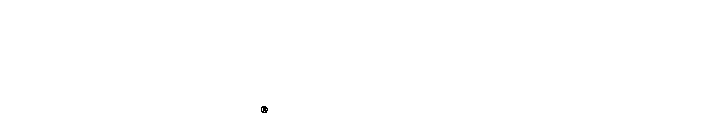
\includegraphics[height=.4cm,keepaspectratio]{../shared/Logo_GTCMT_white}
    \end{textblock*}
}


%%%%%%%%%%%%%%%%%%%%%%%%%%%%%%%%%%%%%%%%%%%%%%%%%%%%%%%%%%%%%%%%%%%%%%%%%%%%%%%%%%
\setbeamertemplate{title page}[default][colsep=-4bp,rounded=false,shadow=false]
\setbeamertemplate{title page}
{
    %\begin{textblock*}{100mm}(15cm,.51cm)
            %\href{https://github.com/alexanderlerch/ACA-Slides/blob/2nd_edition/\jobname.pdf}{\includegraphics[height=.5cm,keepaspectratio]{graph/Logo_github}}\hspace*{2ex}
    %\end{textblock*}
    %\begin{textblock*}{100mm}(15cm,1.3cm)
            %\href{\IEEELink}{\includegraphics[height=.5cm,keepaspectratio]{graph/icon/book}}\hspace*{2ex}
    %\end{textblock*}
    \vskip-10ex
    \begin{beamercolorbox}[wd=\paperwidth,ht=.7\paperheight,dp=0.6ex]{frametitle} %35ex
        %\begin{flushright}
            %\href{http://www.gtcmt.gatech.edu}{
\includegraphics[height=.8cm,keepaspectratio]{graph/Logo_GTCMT_black}}\hspace*{2ex}
        %\end{flushright}
        
        \hspace*{1.8ex}\LARGE\inserttitle%
        
        \vspace*{.5ex}
        
        \hspace*{1.3ex}\small\insertsubtitle%
        
        \vspace*{.5ex}
    \end{beamercolorbox}%
    \nointerlineskip%
    \begin{beamercolorbox}[wd=\paperwidth,ht=.4\paperheight,dp=0.6ex]{page number in head/foot}
        %\vspace*{-.5ex}
        \hspace*{1.7ex}\small\insertauthor%
        
        %\hspace*{1.7ex}\small }%
        
        \vspace*{12ex}
        \vfill
        \begin{flushright}
            \href{http://www.gtcmt.gatech.edu}{
\includegraphics[height=.5cm,keepaspectratio]{../shared/Logo_GTCMT_black}}\hspace*{2ex}
        \end{flushright}
    \end{beamercolorbox}%
}


%%%%%%%%%%%%%%%%%%%%%%%%%%%%%%%%%%%%%%%%%%%%%%%%%%%%%%%%%%%%%%%%%%%%%%%%%%%%%%%%%%
%\makeatother
\setbeamertemplate{footline}
{
  \leavevmode%
  \hbox{%
  \begin{beamercolorbox}[wd=.5\paperwidth,ht=2.25ex,dp=1ex,left,leftskip=1ex]{page number in head/foot}%
    \insertsubtitle
  \end{beamercolorbox}%
  \begin{beamercolorbox}[wd=.5\paperwidth,ht=2.25ex,dp=1ex,right,rightskip=1ex]{page number in head/foot}%
    \hfill
    \insertframenumber{} / \inserttotalframenumber
  \end{beamercolorbox}}%
  \vskip0pt%
}
%\makeatletter


%%%%%%%%%%%%%%%%%%%%%%%%%%%%%%%%%%%%%%%%%%%%%%%%%%%%%%%%%%%%%%%%%%%%%%%%%%%%%%%%%%
\beamertemplatenavigationsymbolsempty
\setbeamertemplate{navigation symbols}{}
\setbeamertemplate{blocks}[default]%[rounded=false,shadow=false]
\setbeamertemplate{itemize item}[square]
\setbeamertemplate{itemize subitem}[circle]
\setbeamertemplate{itemize subsubitem}[triangle]
\setbeamertemplate{enumerate item}[square]
\setbeamertemplate{enumerate subitem}[circle]
\setbeamertemplate{enumerate subsubitem}[circle]


%%%%%%%%%%%%%%%%%%%%%%%%%%%%%%%%%%%%%%%%%%%%%%%%%%%%%%%%%%%%%%%%%%%%%%%%%%%%%%%%%%
% colors
\setbeamercolor{structure}{fg=darkgray}
\setbeamercovered{transparent} %invisible
\setbeamercolor{bibliography entry author}{fg=black}
\setbeamercolor*{bibliography entry title}{fg=black}
\setbeamercolor*{bibliography entry note}{fg=black}
\setbeamercolor{frametitle}{fg=black}
\setbeamercolor{title}{fg=white}
\setbeamercolor{subtitle}{fg=white}
\setbeamercolor{frametitle}{fg=white}
\setbeamercolor{framesubtitle}{fg=white}
\setbeamercolor{mini frame}{fg=white, bg=black}
\setbeamercolor{section in head/foot}{fg=white, bg=darkgray}
\setbeamercolor{page number in head/foot}{fg=black, bg=gtgold}
\setbeamercolor{item projected}{fg=white, bg=black}

%---------------------------------------------------------------------------------

%%%%%%%%%%%%%%%%%%%%%%%%%%%%%%%%%%%%%%%%%%%%%%%%%%%%%%%%%%%%%%%%%%%%%%%%%%%%%%%%%%
%%%%%%%%%%%%%%%%%%%%%%%%%%%%%%%%%%%%%%%%%%%%%%%%%%%%%%%%%%%%%%%%%%%%%%%%%%%%%%%%%%
% title information
\title[]{MUSI6202: Digital Signal Processing for Music}   
\author[alexander lerch]{alexander lerch} 
%\institute{~}
%\date[Alexander Lerch]{}
%\titlegraphic{\vspace{-16mm}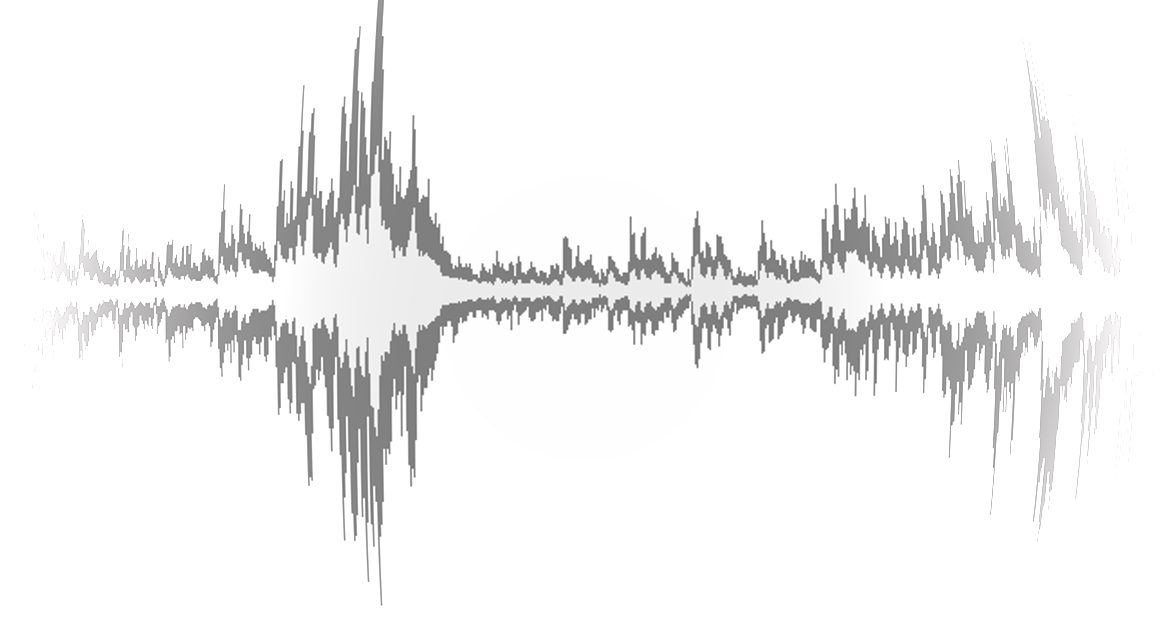
\includegraphics[width=\textwidth,height=3cm]{title}}

%%%%%%%%%%%%%%%%%%%%%%%%%%%%%%%%%%%%%%%%%%%%%%%%%%%%%%%%%%%%%%%%%%%%%%%%%%%%%%%%%%
%%%%%%%%%%%%%%%%%%%%%%%%%%%%%%%%%%%%%%%%%%%%%%%%%%%%%%%%%%%%%%%%%%%%%%%%%%%%%%%%%%
% colors
\definecolor{gtgold}{rgb}{.914, .664, 0} %0e7eed {rgb}{0.88,0.66,1,0.06} [234, 170, 0]/256 %96caff
\definecolor{darkgray}{rgb}{.15, .15, .15}
\definecolor{lightblue}{HTML}{0e7eed}
\definecolor{highlight}{rgb}{0, 0, 1} %_less!40

%%%%%%%%%%%%%%%%%%%%%%%%%%%%%%%%%%%%%%%%%%%%%%%%%%%%%%%%%%%%%%%%%%%%%%%%%%%%%%%%%%
%%%%%%%%%%%%%%%%%%%%%%%%%%%%%%%%%%%%%%%%%%%%%%%%%%%%%%%%%%%%%%%%%%%%%%%%%%%%%%%%%%
% relative paths
\graphicspath{{../graph/}}


%%%%%%%%%%%%%%%%%%%%%%%%%%%%%%%%%%%%%%%%%%%%%%%%%%%%%%%%%%%%%%%%%%%%%%%%%%%%%%%%%%
%%%%%%%%%%%%%%%%%%%%%%%%%%%%%%%%%%%%%%%%%%%%%%%%%%%%%%%%%%%%%%%%%%%%%%%%%%%%%%%%%%
% units
\setlength{\unitlength}{1mm}

%%%%%%%%%%%%%%%%%%%%%%%%%%%%%%%%%%%%%%%%%%%%%%%%%%%%%%%%%%%%%%%%%%%%%%%%%%%%%%%%%%
%%%%%%%%%%%%%%%%%%%%%%%%%%%%%%%%%%%%%%%%%%%%%%%%%%%%%%%%%%%%%%%%%%%%%%%%%%%%%%%%%%
% math
\DeclareMathOperator*{\argmax}{argmax}
\DeclareMathOperator*{\argmin}{argmin}
\DeclareMathOperator*{\atan}{atan}
\DeclareMathOperator*{\arcsinh}{arcsinh}
\DeclareMathOperator*{\sign}{sign}
\DeclareMathOperator*{\tcdf}{tcdf}
\DeclareMathOperator*{\si}{sinc}
\DeclareMathOperator*{\princarg}{princarg}
\DeclareMathOperator*{\arccosh}{arccosh}
\DeclareMathOperator*{\hwr}{HWR}
\DeclareMathOperator*{\flip}{flip}
\DeclareMathOperator*{\sinc}{sinc}
\DeclareMathOperator*{\floor}{floor}
\newcommand{\e}{{e}}
\newcommand{\jom}{\mathrm{j}\omega}
\newcommand{\jOm}{\mathrm{j}\Omega}
\newcommand   {\mat}[1]    		{\boldsymbol{\uppercase{#1}}}		%bold
\renewcommand {\vec}[1]    		{\boldsymbol{\lowercase{#1}}}		%bold

%%%%%%%%%%%%%%%%%%%%%%%%%%%%%%%%%%%%%%%%%%%%%%%%%%%%%%%%%%%%%%%%%%%%%%%%%%%%%%%%%%
%%%%%%%%%%%%%%%%%%%%%%%%%%%%%%%%%%%%%%%%%%%%%%%%%%%%%%%%%%%%%%%%%%%%%%%%%%%%%%%%%%
% media9
\newcommand{\includeaudio}[1]{
\href{run:audio/#1.mp3}{
\includegraphics[width=5mm, height=5mm]{graph/SpeakerIcon}}}

\newcommand{\includeanimation}[4]{{\begin{center}
                        \animategraphics[autoplay,loop,scale=.7]{#4}{animation/#1-}{#2}{#3}        
                        \end{center}
                        \addreference{matlab source: \href{https://github.com/alexanderlerch/ACA-Plots/blob/master/matlab/animate#1.m}{matlab/animate#1.m}}}
                        \inserticon{video}}
                        
%%%%%%%%%%%%%%%%%%%%%%%%%%%%%%%%%%%%%%%%%%%%%%%%%%%%%%%%%%%%%%%%%%%%%%%%%%%%%%%%%%
%%%%%%%%%%%%%%%%%%%%%%%%%%%%%%%%%%%%%%%%%%%%%%%%%%%%%%%%%%%%%%%%%%%%%%%%%%%%%%%%%%
% other commands
\newcommand{\question}[1]{%\vspace{-4mm}
                          \setbeamercovered{invisible}
                          \begin{columns}[T]
                            \column{.9\textwidth}
                                \textbf{#1}
                            \column{.1\textwidth}
                                \vspace{-8mm}
                                \begin{flushright}
                                     
\includegraphics[width=.9\columnwidth]{graph/question_mark}
                                \end{flushright}
                                \vspace{6mm}
                          \end{columns}\pause\vspace{-12mm}}

\newcommand{\toremember}[1]{
                        \inserticon{lightbulb}
                        }

\newcommand{\matlabexercise}[1]{%\vspace{-4mm}
                          \setbeamercovered{invisible}
                          \begin{columns}[T]
                            \column{.8\textwidth}
                                \textbf{matlab exercise}: #1
                            \column{.2\textwidth}
                                \begin{flushright}
                                     \includegraphics[scale=.5]{graph/logo_matlab}
                                \end{flushright}
                                %\vspace{6mm}
                          \end{columns}}

\newcommand{\addreference}[1]{  
                  
                    \begin{textblock*}{\baselineskip }(.98\paperwidth,.5\textheight) %(1.15\textwidth,.4\textheight)
                         \begin{minipage}[b][.5\paperheight][b]{1cm}%
                            \vfill%
                             \rotatebox{90}{\tiny {#1}}
                        \end{minipage}
                   \end{textblock*}
                    }
                    
\newcommand{\figwithmatlab}[1]{
                    \begin{figure}
                        \centering
                        \includegraphics[scale=.7]{#1}
                        %\label{fig:#1}
                    \end{figure}
                    
                    \addreference{matlab source: \href{https://github.com/alexanderlerch/MUSI-6202/blob/main/matlab/plot#1.m}{plot#1.m}}}
\newcommand{\figwithref}[2]{
                    \begin{figure}
                        \centering
                        \includegraphics[scale=.7]{#1}
                        \label{fig:#1}
                    \end{figure}
                    
                    \addreference{#2}}  
                                    
\newcommand{\inserticon}[1]{
                    \begin{textblock*}{100mm}(14.5cm,7.5cm)
                        \includegraphics[height=.8cm,keepaspectratio]{graph/#1}
                    \end{textblock*}}            

%%%%%%%%%%%%%%%%%%%%%%%%%%%%%%%%%%%%%%%%%%%%%%%%%%%%%%%%%%%%%%%%%%%%%%%%%%%%%%%%%%
%%%%%%%%%%%%%%%%%%%%%%%%%%%%%%%%%%%%%%%%%%%%%%%%%%%%%%%%%%%%%%%%%%%%%%%%%%%%%%%%%%
% counters
\newcounter{i}
\newcounter{j}
\newcounter{iXOffset}
\newcounter{iYOffset}
\newcounter{iXBlockSize}
\newcounter{iYBlockSize}
\newcounter{iYBlockSizeDiv2}
\newcounter{iXBlockSizeDiv2}
\newcounter{iDistance}

\newcommand{\IEEELink}{https://ieeexplore.ieee.org/servlet/opac?bknumber=9965970}

\addbibresource{../shared/references}



\subtitle{Part 22: Time-stretching and Pitch-shifting}

%%%%%%%%%%%%%%%%%%%%%%%%%%%%%%%%%%%%%%%%%%%%%%%%%%%%%%%%%%%%%%%%%%%%%%%%%%%%
\begin{document}
    % generate title page
	\title[]{Digital Signal Processing for Music}   
\author[alexander lerch]{alexander lerch} 
%\institute{~}
%\date[Alexander Lerch]{}
\titlegraphic{\vspace{-16mm}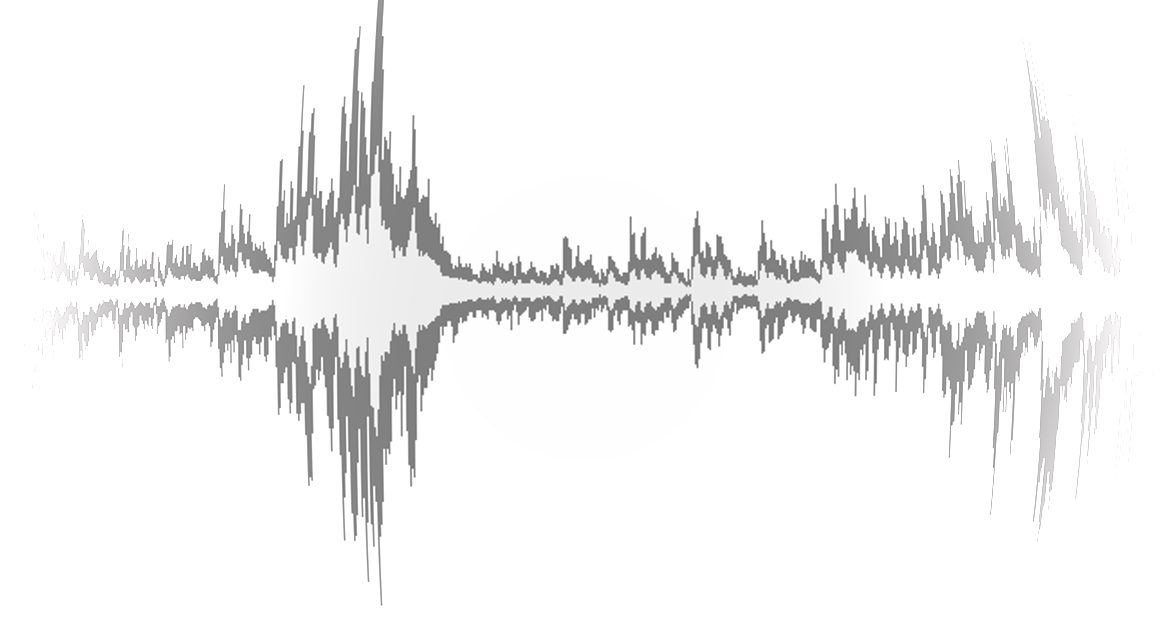
\includegraphics[width=\textwidth,height=3cm]{title}}


\begin{frame}
    \titlepage
    %\vspace{-5mm}
    \begin{flushright}
        \href{http://www.gtcmt.gatech.edu}{
\includegraphics[height=.8cm,keepaspectratio]{../shared/Logo_GTCMT_black}}
    \end{flushright}
\end{frame}


\section[intro]{introduction}
\begin{frame}\frametitle{time stretching \& pitch shifting}\framesubtitle{introduction}
	\begin{itemize}
		\item	\textbf{time stretching}\\
			change playback speed/tempo without changing pitch
		\pause
        \bigskip
		\item	\textbf{pitch shifting}\\
			change pitch without changing tempo/playback speed
		\pause
        \bigskip
		\item	\textbf{terms}
            \begin{itemize}
                \item   time/pitch scaling
                \item   time expansion/compression
            \end{itemize}
	\end{itemize}

\end{frame}

\begin{frame}\frametitle{time stretching \& pitch shifting}\framesubtitle{applications}
	\begin{itemize}
		\item	\textbf{beat matching}: align tempo of two or more audio files (mashup)
		\pause
        \smallskip
		\item	\textbf{key lock}: ``align'' pitch of two or more audio files (mashup)
		\pause
        \smallskip
		\item	\textbf{pitch/time correction}: edit intonation, frequency deviation, vibrato, glissando
		\pause
        \smallskip
		\item	video \textbf{frame rate conversion}
		\pause
        \smallskip
		\item	\textbf{sample player/libraries}
		\pause
        \smallskip
		\item	\textbf{sound design}
		\pause
        \smallskip
		\item	\textbf{educational software}: pitch and timing visualization
	\end{itemize}
\end{frame}

\section[basics]{fundamentals}
\begin{frame}\frametitle{time stretching \& pitch shifting}\framesubtitle{stretch and pitch factors}
	\begin{eqnarray*}
		s	&=& \frac{t_{output}}{t_{input}}\\
		p	&=& \frac{f_{output}}{f_{input}}
	\end{eqnarray*}
	\pause
	\textbf{examples}:
	\begin{itemize}
		\item	\textit{half speed}: 
			\pause
			$s = 2$
		\pause
		\item	\textit{half pitch}: 
			\pause
			$p = \frac{1}{2}$
		\pause
		\item	\textit{semitone up/down}: 
			\pause
			\begin{equation}
				p_u = 2^{\nicefrac{1}{12}} = 1.059\quad p_d = 2^{-\nicefrac{1}{12}} = 0.9439\nonumber
			\end{equation}
		\pause
		\item	\textit{\unit[100]{BPM} $\rightarrow$ \unit[75]{BPM}}: 
			\pause
			$s = \frac{4}{3}$
	\end{itemize}
\end{frame}
    \begin{frame}{time stretching \& pitch shifting}{resampling}
        \begin{itemize}
            \item   \textbf{traditional}: resampling
                \begin{itemize}
                    \item   change inter-sample 'distance' by \textbf{interpolation}
                    \item   keep \textbf{playback sample rate constant}
                    \pause
                    \bigskip
                    \item   audio example
                    \uncover<2->{
                        \begin{itemize}
                            \item   original \includeaudio{cathy}
                            \item   resample \includeaudio{cathyResample}
                        \end{itemize}
                        }
                    \pause
                    \bigskip 
                    \item[$\Rightarrow$] tempo change results in pitch change (and vice versa)
                    \begin{equation*}
                        s = \frac{1}{p}
                    \end{equation*}
                \end{itemize}
        \end{itemize}
    \end{frame}
 
\begin{frame}\frametitle{time stretching \& pitch shifting}\framesubtitle{stretching: frequency domain}
		\begin{figure}
			\centerline{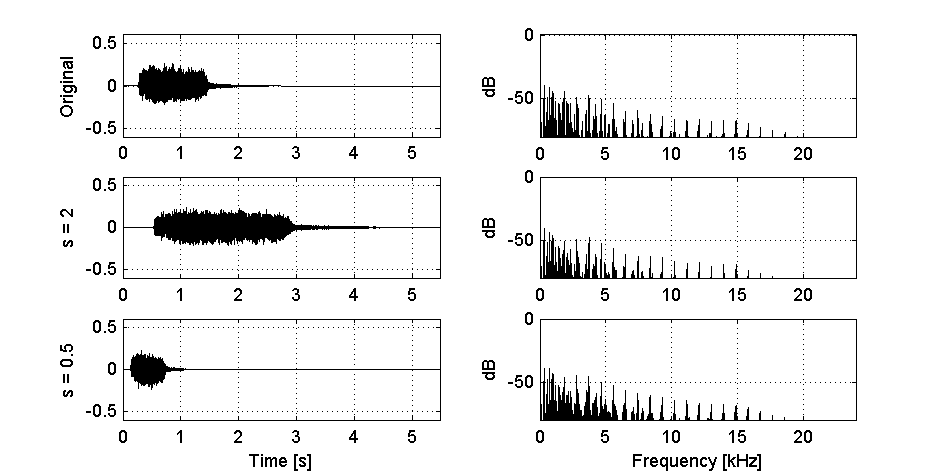
\includegraphics[scale=.7]{graph/fx4_timestretchintro}}
		\end{figure}
\end{frame}
   
    \section[ola]{time-segment processing (ola)}
    \begin{frame}{OLA}{introduction}
        overlap and add approaches for, e.g.,
        
        \begin{itemize}
            \item   granular synthesis
            \item   time/frequency synthesis and processing
            \item   {\color<2->{gtgold}time-stretching and pitch-shifting}
        \end{itemize}
    \end{frame}

    \begin{frame}{OLA}{time stretching}
            \textbf{overlap and add}
            \begin{enumerate}
                \item	\textbf{split input} signal into overlapping blocks
                \pause
                \item	\textbf{duplicate or discard blocks} depending on stretch factor
                %\item[] \includemovie[poster=graph/SpeakerIcon.png,mouse=true]{5mm}{5mm}{cathyOLAout} $s = \nicefrac{4}{3}$
            \end{enumerate}
            \uncover<2->{
            \vspace{-5mm}
            \begin{columns}
                \column{.6\linewidth}
                    \begin{figure}
                        \centering
                        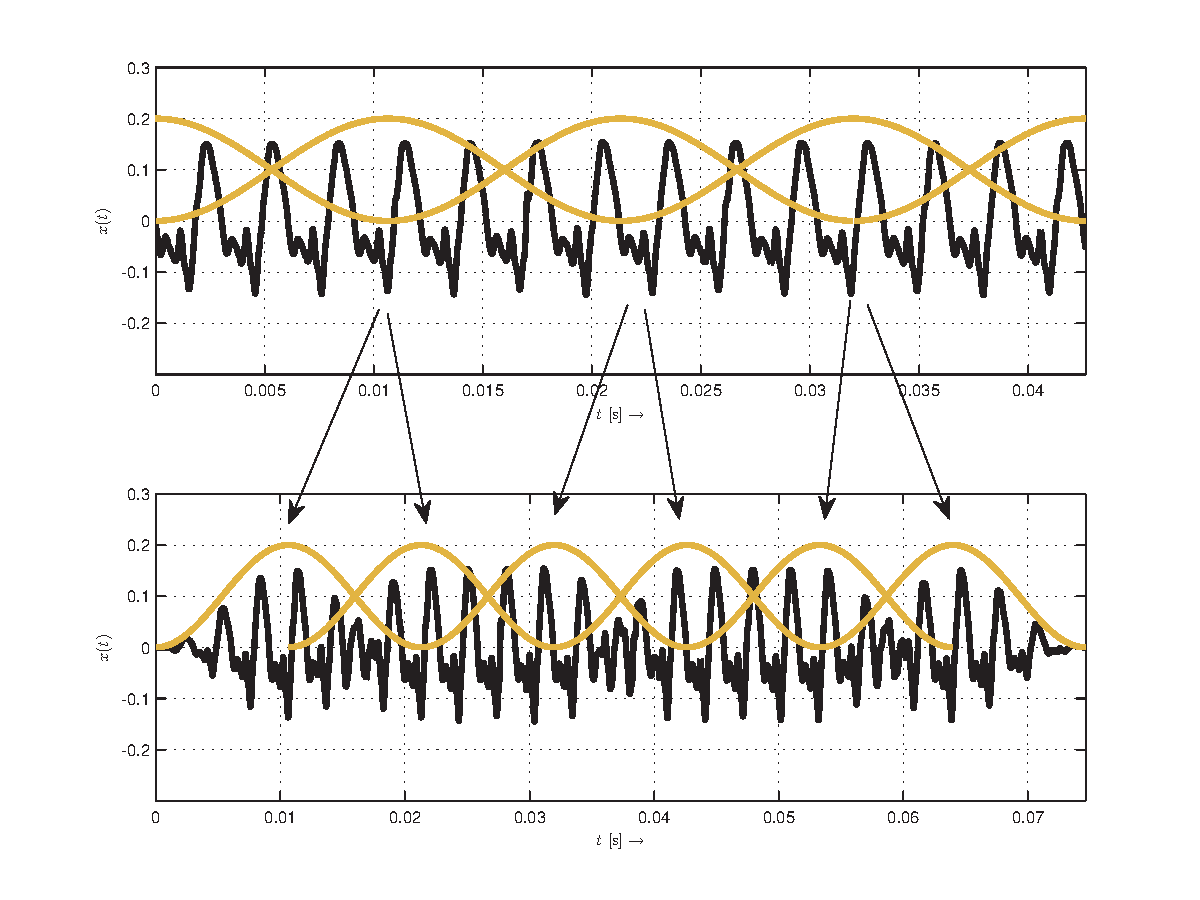
\includegraphics[scale=.3]{graph/OLA}
                    \end{figure}\vspace{-5mm}

                \column{.4\linewidth}
                    \vspace{10mm}
                    \begin{itemize}
                        \item   \includeaudio{cathy}\; orig
                        \item  \includeaudio{cathyOLAout}\; $s =\nicefrac{4}{3}$ 
                    \end{itemize}
            \end{columns}
            }
    \end{frame}

    \begin{frame}{PSOLA}{time stretching}
            \textbf{pitch synchronous overlap and add}
            \begin{itemize}
                \item   use the OLA principle, but
                \item	\textbf{adapt block length} to fundamental period length
            \end{itemize}
            \only<1>{
            \begin{figure}
                \centerline{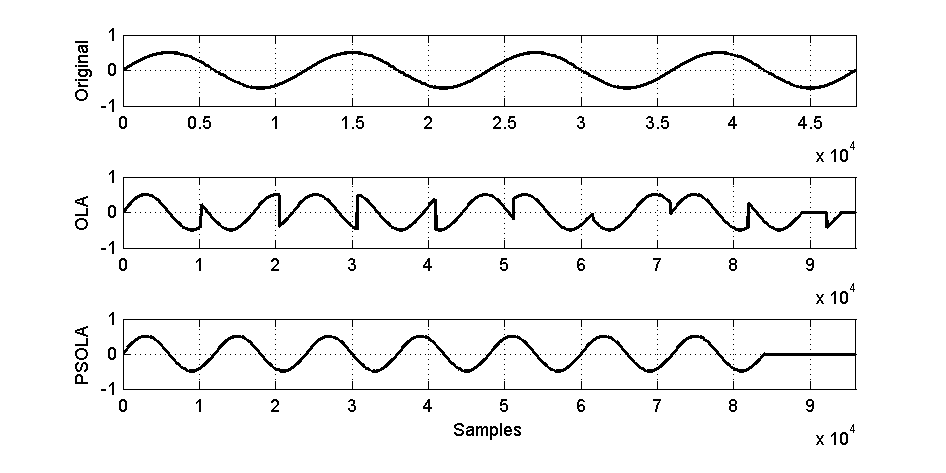
\includegraphics[scale=.6]{graph/fx4_olapsola}}
                \label{fig:fx4_olapsola}
            \end{figure}
            }          
            \pause
            \begin{columns}
                \column{.6\linewidth}
                    \begin{figure}
                        \centering
                        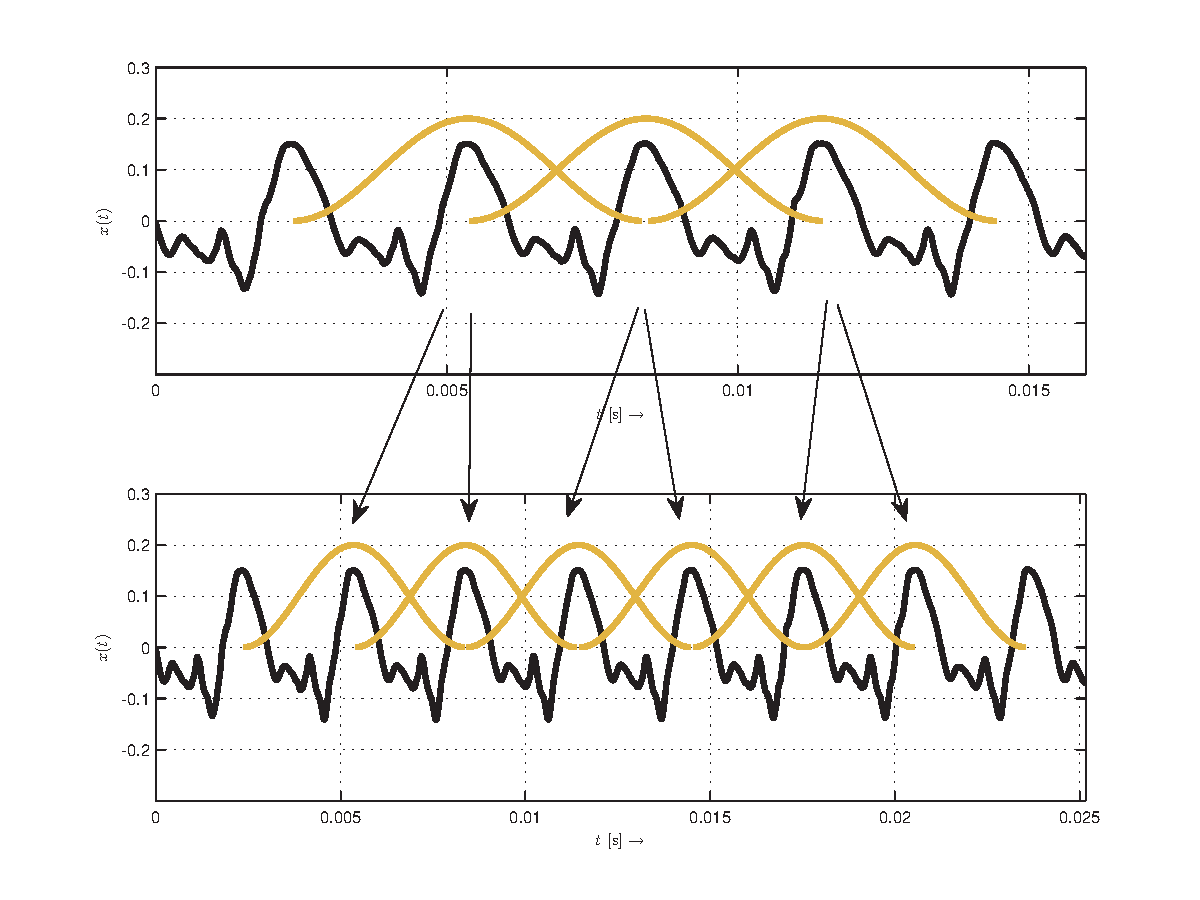
\includegraphics[scale=.3]{graph/PSOLA.pdf}
                    \end{figure}\vspace{-5mm}
                \column{.4\linewidth}
                    \vspace{10mm}
                    \begin{itemize}
                        \item   \includeaudio{cathy}\; orig
                        \item \includeaudio{cathySOLout}\; $s = \nicefrac{4}{3}$ 
                    \end{itemize}
            \end{columns}
            \vspace{50mm}
    \end{frame}
\begin{frame}{PSOLA}{transient copying}
				\begin{figure}
					\centerline{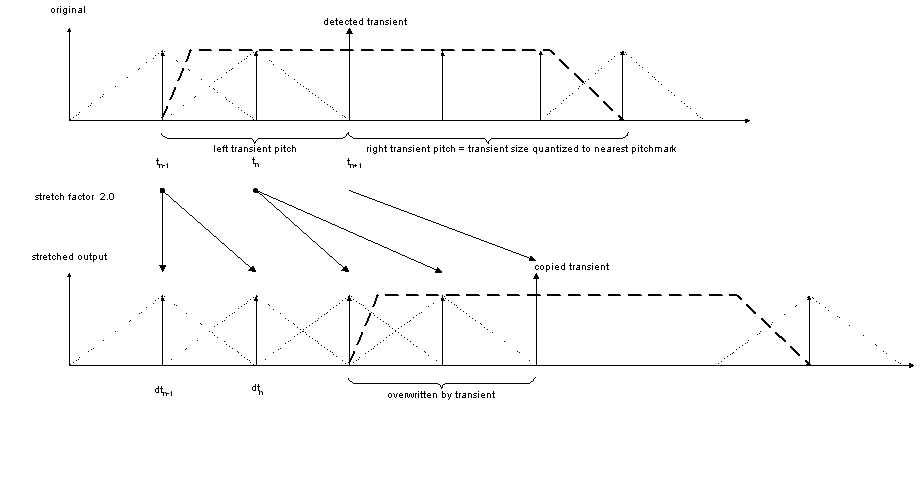
\includegraphics[scale=.3]{graph/transcpy}}
				\end{figure}
\end{frame}

    \begin{frame}{PSOLA}{time stretching summary}
        \vspace{-3mm}
        \begin{itemize}
            \item   \textbf{processing steps}
                \begin{enumerate}
                    \item   detect \textit{fundamental frequency}/period length
                    \item   set \textit{pitch marks}
                    \item   intelligently \textit{select blocks} to be repeated/discarded
                \end{enumerate}
            \pause
            \item   \textbf{advantages}
                \begin{itemize}
                    \item   \textit{high granularity} --- modify audio on period length resolution
                    \item   \textit{high quality}
                \end{itemize}
            \pause
            \item   \textbf{problems}
                \begin{itemize}
                    \item   quality depends on \textit{pitch tracking} reliability
                    \item   quality and timbre depends on \textit{pitch mark positioning}
                    \item   works only for \textit{monophonic} input signals
                        \begin{itemize}
                            \item   polyphonic and noisy segments
                            \item reverberation and overlapping tones
                        \end{itemize}
                   \item    \textit{noise, plosives} require special consideration
                   \item    \textit{copying} artifacts (double transients, timing deviations)
                \end{itemize}
            \pause
            \item   \textbf{typical applications}
                \begin{itemize}
                    \item   \textbf{standard approach for vocal editing tools}
                \end{itemize}
        \end{itemize}
    \end{frame}

\section{phase vocoder}

    \begin{frame}{time stretching}{phase vocoder}
        \begin{enumerate}
            \item	\textbf{split input} signal into overlapping blocks
            \item<2->	compute \textbf{magnitude and phase spectrum} of each block
            \item<3->	\textbf{change overlap ratio} between blocks depending on stretch factor
            \item<4->	keep the magnitude, \textbf{adapt the phase per bin} to the block's new time stamp
        \end{enumerate}
        
        \begin{columns}
            \column{6cm}\vspace{-8mm}
                \begin{figure}
                    \begin{picture}(80,30)
                        \setcounter{iYOffset}{30}
                        \put(0, \value{iYOffset}){\tiny{\textcolor{gtgold}{input signal}}}
                        \setcounter{iXOffset}{0}
                        \addtocounter{iYOffset}{-3}
                        
                        \only<1->
                        {    
                            \put(\value{iXOffset}, \value{iYOffset}){\framebox(36, 2)}    

                            \addtocounter{iYOffset}{-2}
                            \setcounter{i}{1}
                            \whiledo{\value{i}<6}	
                            {
                                \put(\value{iXOffset}, \value{iYOffset}){\framebox(16, .5)}
                                \dottedline{.5}(\value{iXOffset}, \value{iYOffset})(\value{iXOffset},29)
                                \addtocounter{iXOffset}{5}
                                \addtocounter{iYOffset}{-1}
                                \stepcounter{i} 
                            }	
                        }
                        \only<2->
                        {    
                            \put(15,18){{$\Downarrow$}}
                            
                            \put(47,16){\ovalbox{\tiny{\parbox{20mm}{\centering{STFT\\ magnitude \& phase}}}}}
                        }
                        
                        \only<3->
                        {    
                            \setcounter{iXOffset}{0}
                            \setcounter{iYOffset}{14}
                            \setcounter{i}{1}                            
                            \whiledo{\value{i}<6}	
                            {
                                \put(\value{iXOffset}, \value{iYOffset}){\framebox(16, .5)}
                                %\dashline{4}(0,11)(60,11)
                                \dottedline{.5}(\value{iXOffset}, \value{iYOffset})(\value{iXOffset},2)
                                \addtocounter{iXOffset}{7}
                                \addtocounter{iYOffset}{-1}
                                \stepcounter{i} 
                            }	
                            \addtocounter{iYOffset}{-3}
                        }
                        \only<4->
                        {    
                            \put(15,6){{$\Downarrow$}}
                            \put(47,6){\ovalbox{\tiny{\parbox{20mm}{\centering{phase extrapol. \\ window comp.}}}}}
                        }
                        
                        \only<5->
                        {    
                            \put(0, 2){\framebox(44, 2)}    
                            \put(0, 0){\tiny{\textcolor{gtgold}{output signal}}}
                        }
                    \end{picture}
                \end{figure}

            \column{4cm}\vspace{-20mm}
                    \vspace{20mm}
                \only<4>
                {
                     \begin{figure}
                        \centering
                        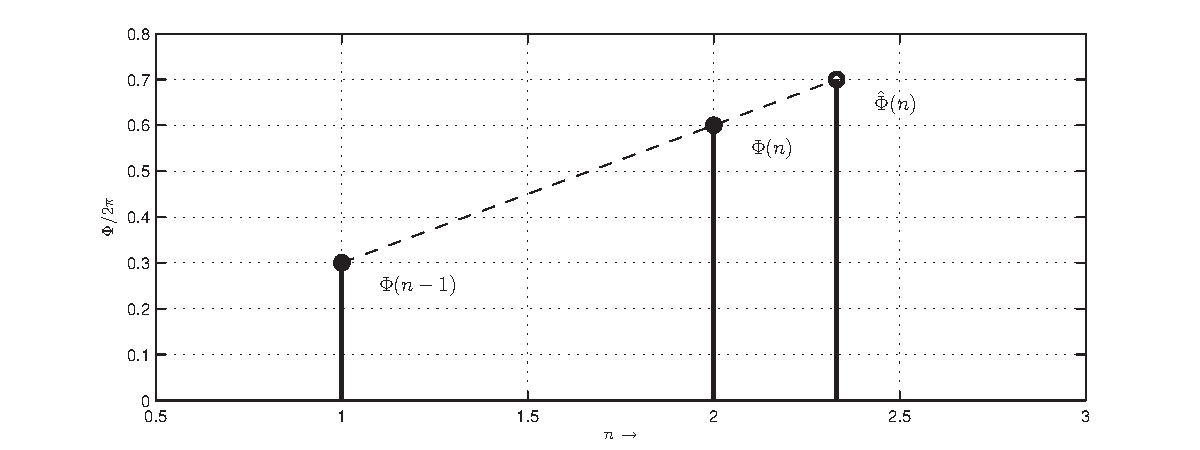
\includegraphics[scale=.25]{graph/phaseextrapol.pdf}
                     \end{figure}
                }
                \only<5->
                {
                    \begin{itemize}
                        \item   \includeaudio{cathy}\; original 
                        \item   \includeaudio{cathypvout}\; pv $s = \nicefrac{4}{3}$ 
                    \end{itemize}
                }
        \end{columns}
        \vspace{50mm}
    \end{frame}

        \begin{frame}{time stretching}{frequency reassignment: relation of phase and frequency 1/2}
            \begin{columns}
            \column{.5\linewidth}
            \vspace{-10mm}
            \includeanimation
                {Phasor}
                {00}
                {160}
                {10}
            \column{.5\linewidth}
           \begin{itemize}
                \item   phasor representation:
                    \begin{enumerate}
                        \item   sine value is defined by magnitude and phase
                        \item   decreasing the amplitude $\Rightarrow$ shorter vector
                        \item   increasing the frequency $\Rightarrow$ increasing speed
                    \end{enumerate}
            \end{itemize}
            \end{columns}
                        \addreference{matlab source: \href{https://github.com/alexanderlerch/ACA-Slides/blob/master/matlab/animatePhasor.m}{matlab/animatePhasor.m}}
            \inserticon{video}
        \end{frame}
        \begin{frame}{time stretching}{frequency reassignment: relation of phase and frequency 2/2}

            \begin{columns}
            \column{0.3\textwidth}
            
            \begin{figure}
                \begin{tiny}
                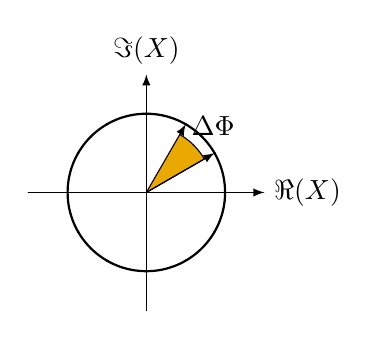
\begin{tikzpicture}[scale=1,cap=round,>=latex]
                    % draw the coordinates
                    \draw[->] (-1.5cm,0cm) -- (1.5cm,0cm) node[right,fill=white] {$\Re(X)$};
                    \draw[->] (0cm,-1.5cm) -- (0cm,1.5cm) node[above,fill=white] {$\Im(X)$};
        
                    \draw[fill=gtgold] (0,0) -- (30:.85cm) arc (30:60:.85cm);
                    \draw (45:1.2cm) node {$\Delta\Phi$};
                    \draw[->] (0cm,0cm) -- (0.8660cm,0.5cm);
                    \draw[->] (0cm,0cm) -- (0.5cm,0.8660cm);
        
                    % draw the unit circle
                    \draw[thick] (0cm,0cm) circle(1cm);
            
                    \foreach \x in {0,30,...,360} {
        %	                % dots at each point
                            \filldraw[black] (\x:1cm) circle(0.2pt);
                    }
                \end{tikzpicture}
                \end{tiny}
            \end{figure}
             \column{0.7\textwidth}
            \begin{itemize}
                \item   frequency and phase change closely related:
                    \begin{itemize}
                        \item<2-> time for full rotation is period length $T$ with \[f = \frac{1}{T}\]
                        \item<3-> time for fractional rotation $\Delta\Phi$ is corresponding fraction of period length \[f = \frac{\Delta\Phi}{\Delta t}\]
                        \item<4-> in other words: 
                        \begin{eqnarray*}
                            \Phi(t) &=& \omega\cdot t\\
                            \Rightarrow \frac{d\Phi(t)}{dt} &=& \omega = 2\pi f
                        \end{eqnarray*}
                    \end{itemize}
            \end{itemize}
            \end{columns}
        \end{frame}
        \begin{frame}{time stretching}{frequency reassignment: principles}
            frequency domain:
            \begin{itemize}
                \item   instead of using the bin frequency
                    \[ f(k) = k*\frac{f_\mathrm{S}}{\mathcal{K}}\]
                \item   we use the phase of each bin $\Phi(k,n)$
                \item   to compute the frequency from the phase difference of neighboring blocks
                    \begin{equation*}\label{eq:phasediff}
                        \omega_{\mathrm{I}}(k,n)	\propto \Phi(k,n)-\Phi(k,n-1)
                    \end{equation*}
                \item<2->   $\omega_{\mathrm{I}}(k,n)$ is called \textbf{instantaneous frequency} per block per bin
            \end{itemize}
        \end{frame}
        \begin{frame}{time stretching}{frequency reassignment: scaling factor}
            \begin{itemize}
                \item instantaneous frequency calculation has to take into account
                    \begin{itemize}
                        \item   hop size $\mathcal{H}$
                        \item   sample rate $f_\mathrm{S}$
                    \end{itemize}
                
                    \begin{equation*}
                        \omega_{\mathrm{I}}(k,n) = \frac{\Delta\Phi_{\mathrm{u}}(k,n)}{\mathcal{H}}\cdot f_{\mathrm{S}} 
                    \end{equation*}
                \item<2-> problem: phase ambiguity
                    \begin{equation*}
                        \Phi(k,n) = \Phi(k,n) + j\cdot 2\pi
                    \end{equation*}
                \item<3->[$\Rightarrow$] \textit{phase unwrapping}
            \end{itemize}
        \end{frame}
        \begin{frame}{time stretching}{frequency reassignment: phase unwrapping}

            \begin{enumerate}
                \item	compute unwrapped phase $\Phi_{\mathrm{u}}(k,n)$ 
                        \begin{itemize}
                            \item	estimate unwrapped bin phase
                                    \begin{footnotesize}
                                    \begin{equation*}\label{eq:phi_est}
                                        \hat{\Phi}(k,n) = \Phi(k,n-1) + \underbrace{2\pi k\cdot\frac{\mathcal{H}}{\mathcal{K}}}_{=\omega_k\cdot\frac{\mathcal{H}}{f_\mathrm{s}}} 
                                    \end{equation*}
                                    \end{footnotesize}

                            \item<2->	unwrap phase by shifting current phase to estimate's range
                                    \begin{footnotesize}
                                    \begin{equation*}
                                        \Phi_{\mathrm{u}}(k,n) = \hat{\Phi}(k,n) + \princarg\left[ \Phi(k,n) - \hat{\Phi}(k,n) \right]
                                    \end{equation*}
                                    \end{footnotesize}
                        \end{itemize}

                \item<3->	compute unwrapped phase difference
                        \begin{footnotesize}
                        \begin{eqnarray*}
                            \Delta\Phi_{\mathrm{u}}(k,n)	&=& \Phi_{\mathrm{u}}(k,n) - \Phi(k,n-1)\nonumber\\
                                                \pause
                                                &=& \hat{\Phi}(k,n) + \princarg\left[ \Phi(k,n) - \hat{\Phi}(k,n) \right] - \Phi(k,n-1)\nonumber \\
                                                \pause
                                                &=& \frac{2\pi k}{\mathcal{K}}\mathcal{H} + \princarg\left[ \Phi(k,n) - \Phi(k,n-1) - \frac{2\pi k}{\mathcal{K}}\mathcal{H} \right]\nonumber
                        \end{eqnarray*}
                        \end{footnotesize}
            \end{enumerate}
        
        \end{frame}
        \begin{frame}{time stretching}{frequency reassignment: problems}
                \begin{itemize}
                    \item   \textbf{overlapping spectral components}
                        \begin{itemize}
                            \item   sinusoidal components often overlap (spectral leakage, several instruments playing the same pitch, ...)
                            \smallskip
                                \begin{itemize}
                                    \item[$\Rightarrow$] incorrect phase estimate
                                    \smallskip
                                    \item<2-> increase STFT length to make spectrum as sparse as possible
                                \end{itemize}
                        \end{itemize}
                    \bigskip
                    \item<3->   \textbf{inaccurate phase unwrapping} 
                        \begin{itemize}
                            \item   unwrapping algorithm is based on assumption of similarity between predicted and measured phase
                            \smallskip
                                \begin{itemize}
                                    \item[$\Rightarrow$] incorrect phase estimate
                                    \smallskip
                                    \item<2-> decrease hop size to make time steps as close as possible
                                \end{itemize}
                        \end{itemize}
                \end{itemize}
        \end{frame}
        \begin{frame}{time stretching}{frequency reassignment: example}
            \figwithmatlab{InstantaneousFreq}
        \end{frame}


    \begin{frame}\frametitle{time stretching}\framesubtitle{phase vocoder window compensation}
        \begin{figure}
            \centerline{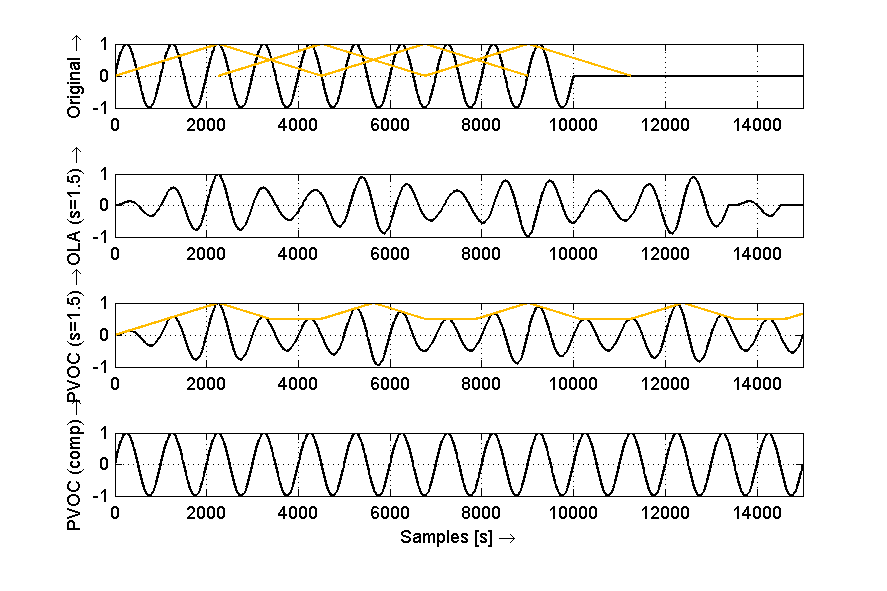
\includegraphics[scale=.7]{graph/pvocIntro}}
        \end{figure}
    \end{frame}

    \begin{frame}{time stretching}{phase vocoder --- properties \& artifacts}
        \begin{itemize}
            \item   \textbf{advantages}:
                \begin{itemize}
                    \item   allows \textit{polyphonic input} (assumption: no overlapping harmonics)
                    \item   absolute \textit{timing stability} (i.e., sample resolution)
                \end{itemize}   
            \pause
            \bigskip
            \item   \textbf{disadvantages}:
                \begin{itemize}
                    \item   \textit{low granularity} --- FFT block size
                    \item   artifacts:
                        \begin{enumerate}
                            \item   phasing
                            \item   transient smearing/doubling
                        \end{enumerate}
                \end{itemize}
        \end{itemize}
    \end{frame}

    \begin{frame}{time stretching}{phase vocoder artifacts: phasing --- spectral leakage 1/3}
        \vspace{-5mm}
        \begin{columns}
        \column{.4\linewidth}
            \begin{figure}
                \centering
                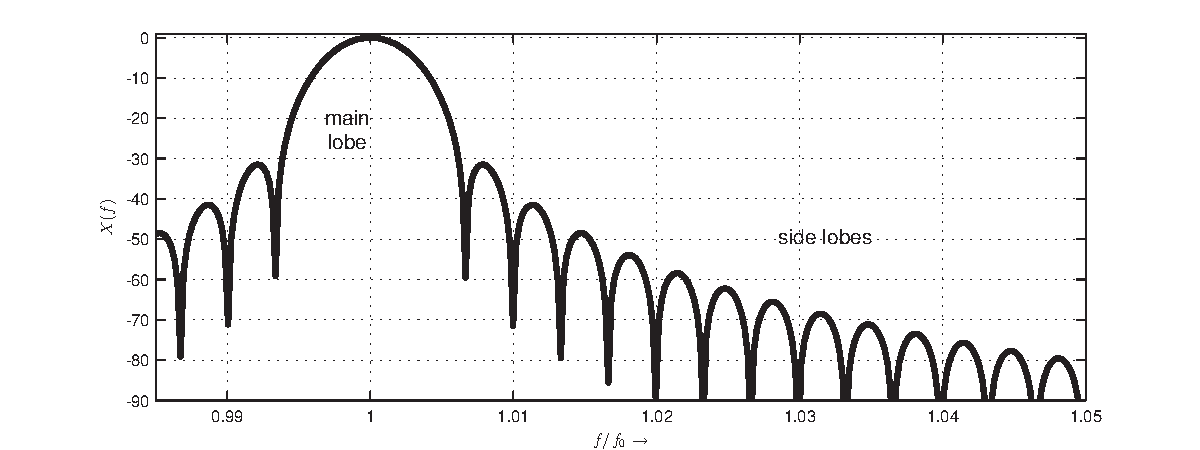
\includegraphics[scale=.3]{graph/SpectralLeakage}
            \end{figure}
        \column{.6\linewidth}
            \begin{figure}
                \centerline{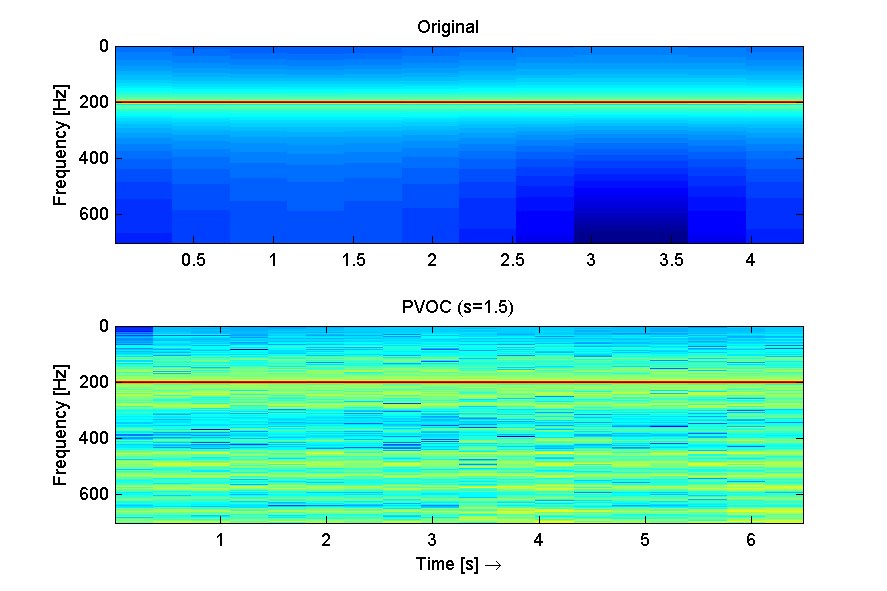
\includegraphics[scale=.5]{graph/PeakSmearingFreq}}
            \end{figure}
        \end{columns}
    \end{frame}
	\begin{frame}{time stretching}{phase vocoder artifacts: phasing --- spectral leakage 2/3}
			\begin{figure}
				\centerline{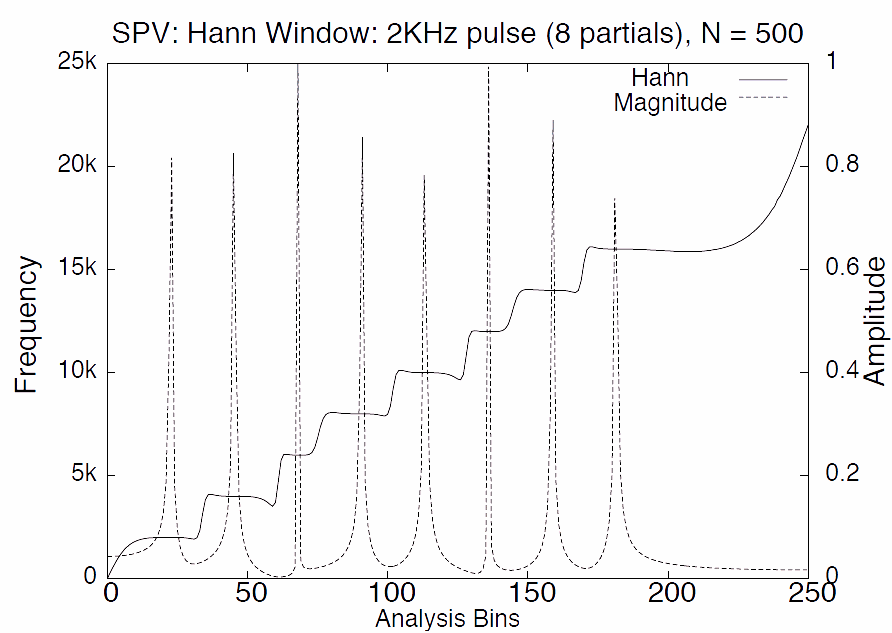
\includegraphics[scale=.4]{graph/instfreq}}
			\end{figure}
    \end{frame}
	\begin{frame}{time stretching}{phase vocoder artifacts: phasing --- spectral leakage 3/3}
                \begin{itemize}
                    \item[$\Rightarrow$] use \textit{frequency reassignment} for grouping and phase sync
                \end{itemize}
                \bigskip
                        \begin{itemize}
                            \item   original  \includeaudio{cathy}
                            \item   pv $s = \nicefrac{4}{3}$ \includeaudio{cathypvout}
                            \item   grouped phase \includeaudio{cathyEffout}
                        \end{itemize}
    \end{frame}
	\begin{frame}{time stretching}{phase vocoder artifacts: phasing --- unsynced harmonics}
        \vspace{-5mm}
        \begin{columns}
        \column{.4\linewidth}
            \begin{figure}
                \centering
                    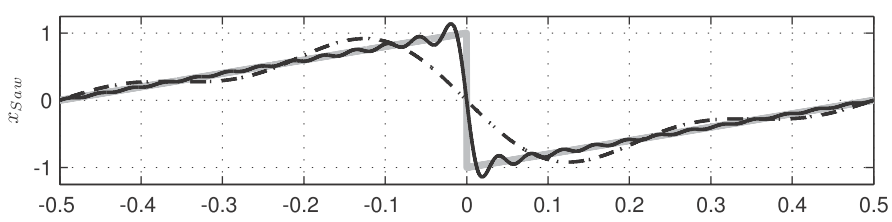
\includegraphics[width=5.3cm,height=2.4cm]{graph/gibbs}
            \end{figure}
        \column{.6\linewidth}
		\only<1>{
            \begin{figure}
                \centerline{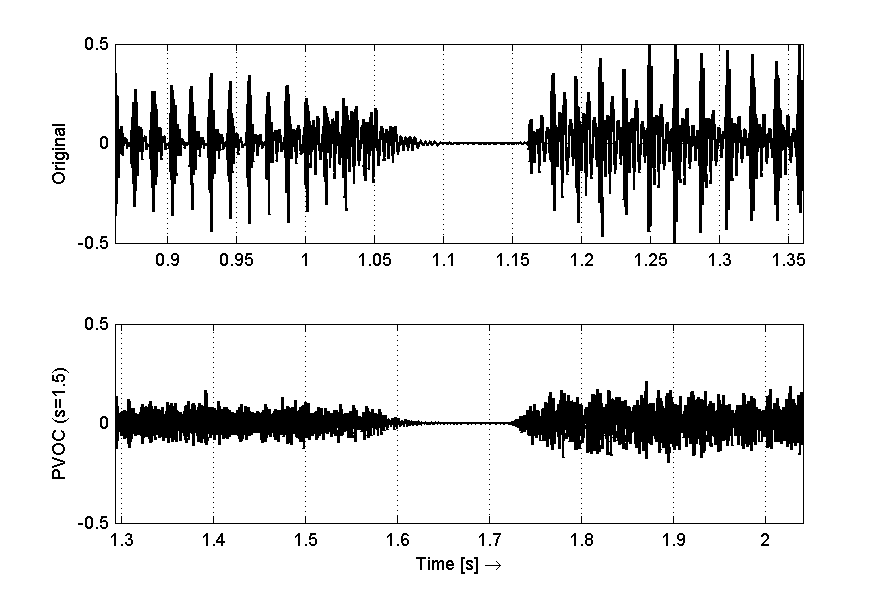
\includegraphics[scale=.5]{graph/phasing}}
            \end{figure}}
            \begin{itemize}
                \item<2->[$\Rightarrow$] use \textit{harmonic analysis} for grouping and phase sync
            \end{itemize}
                    \begin{itemize}
                        \item   original  \includeaudio{cathy}
                        \item   pv $s = \nicefrac{4}{3}$ \includeaudio{cathypvout}
                        \item   synced phase \includeaudio{cathyProout}
                    \end{itemize}
        \end{columns}
    \end{frame}
	\begin{frame}{time stretching}{phase vocoder artifacts: interchannel phasing}
        \begin{itemize}
            \item   phase estimation between channels slightly off due to
                \begin{itemize}
                    \item   numerical inaccuracies (cumulative!)
                    \item   overlapping frequency components
                \end{itemize}
                \pause
                \bigskip
            \item[$\Rightarrow$] change in spatial image
                \begin{itemize}
                            \item   \includeaudio{bigband}\; original  
                            \item   \includeaudio{bigbandPVoc}\; pv $s = \nicefrac{3}{2}$ 
                \end{itemize}
        \end{itemize}
	\end{frame}

    \begin{frame}{time stretching}{phase vocoder artifacts: transient smearing}
        \vspace{-8mm}
        \begin{columns}
            \column{.65\textwidth}
            \vspace{-3mm}
                \begin{figure}
               %     \centering
                    \includegraphics[scale=.35]{graph/TransientSmear}
                \end{figure}

            \column{.3\textwidth}%\vspace{-10mm}
                \begin{itemize}
                \vspace{10mm}
                    \item   \includeaudio{castanets}\; original  
                    \item   \includeaudio{castanetsPVoc}\; pv $s = \nicefrac{3}{2}$ 
                \end{itemize}
        \end{columns}
        \pause
        \vspace{-3mm}
        \begin{itemize}
            \item[$\Rightarrow$] detect transients and \textit{reset phase} per bin
                \begin{itemize}
                    \item   \includeaudio{41_m}\; original  
                    \item   \includeaudio{41pvout}\; pv $s = \nicefrac{4}{3}$ 
                    \item   \includeaudio{41Proout}\; phase reset 
                \end{itemize}
        \end{itemize}
    \end{frame}

\begin{frame}\frametitle{time stretching}\framesubtitle{inherent problems}
	\begin{itemize}
		\item	stretching the audio data can lead to \textbf{``non-natural'' results}
		\pause
        \bigskip
		\item	\textbf{examples}
			\begin{itemize}
				\item tempo dependent \textit{timing variations }
				\pause
				\item	other performance related aspects may get inappropriate lengths and speed: \textit{vibrato, tremolo, glissando}
			\end{itemize}
	\end{itemize}
\end{frame}

\section{pitch shifting}
        \begin{frame}{pitch shifting}{standard approach}
            \begin{itemize}
                \item   \textbf{definition}:\\ change pitch without changing tempo
                \pause
                \item   \textbf{method}:\\ combine stretching and \textit{sample rate conversion} (interpolation)
                    \begin{enumerate}
                        \item   change length with stretching
                        \item   resample to compensate for length difference
                    \end{enumerate}
                \item<2->	\textbf{implementation}: differentiate ``external'' and ``internal'' parameters 
                        \begin{itemize}
                            \item	\textit{extern}: stretch $s_e$ and pitch $p_e$
                            \item	\textit{intern}: stretch $s_i$ and resample $r_i$
                        \end{itemize}
                
                \item<3-> \textbf{example}: pitch shift factor \textbf{$p = \nicefrac{4}{3}$}
					\begin{enumerate}
						\item	\textit{time stretch} (increase length/decrease tempo) $s = \nicefrac{4}{3}$
						\pause
						\item	\textit{resample} (decrease length, increase pitch) $r = \nicefrac{3}{4}$
                        \pause
                        \item[$\Rightarrow$]   audio:
                            \begin{itemize}
                                \item   OLA \includeaudio{cathyOLApitch}
                                \item   phase vocoder \includeaudio{cathypvpitch}
                            \end{itemize}
					\end{enumerate}
            \end{itemize}
        \end{frame}
        \begin{frame}{pitch shifting}{standard approach: stretch, pitch, resample factor examples}
			\setbeamercovered{invisible}

                \begin{itemize}
					\item	extern: $s_e=1$ $p_e=2$
					\pause
					\item[]	intern: $s_i=2$ $r_i=\frac{1}{2}$
					\pause
					\item	extern: $s_e=1$ $p_e=\frac{4}{3}$
					\pause
					\item[]	intern: $s_i=\frac{4}{3}$ $r_i=\frac{3}{4}$
					\pause
					\item	extern: $s_e=\frac{1}{2}$ $p_e=2$
					\pause
					\item[]	intern: $s_i=1$ $r_i=\frac{1}{2}$
					\pause
					\item	extern: $s_e=2$ $p_e=2$
					\pause
					\item[]	intern: $s_i=4$ $r_i=\frac{1}{2}$
				\end{itemize}
  			\setbeamercovered{transparent}
      \end{frame}
        \begin{frame}{pitch shifting}{frequency domain approach}
            \begin{enumerate}
                \item   STFT
                \item<2->   magnitude and phase
                \item<3->   magnitude and instantaneous frequency
                \item<4->   resample both magnitude and frequency spectrum acc.\ to pitch factor
                \item<5->   magnitude and phase
                \item<6->   complex spectrum
                \item<7->   IFFT and OLA
            \end{enumerate}
        \end{frame}
        \subsection{formant preservation}   
        \begin{frame}{pitch shifting}{formant preservation: time domain}
	\begin{itemize}
		\item 	\textbf{idea}
			\begin{itemize}
				\item 	signal is pulse train filtered by transfer function
					\pause
					\begin{itemize}
						\item 	pulse train determines fundamental frequency
						\item	transfer function determines formant shape/timbre characteristics
					\end{itemize}
			\end{itemize}
		\pause
        \bigskip
		\item	\textbf{approach}
			\begin{itemize}
				\item	change grain/pulse distance
				\item	grain ``content'' not modified\\ $\rightarrow$ freq domain not modified
				\pause
                \bigskip
				\item[$\Rightarrow$]	\textbf{``same'' spectrum,\\ different pitch}
			\end{itemize}
	\end{itemize}
    \vspace{-30mm}
        \visible<3->{
                    \begin{flushright}
                        \hspace{10mm}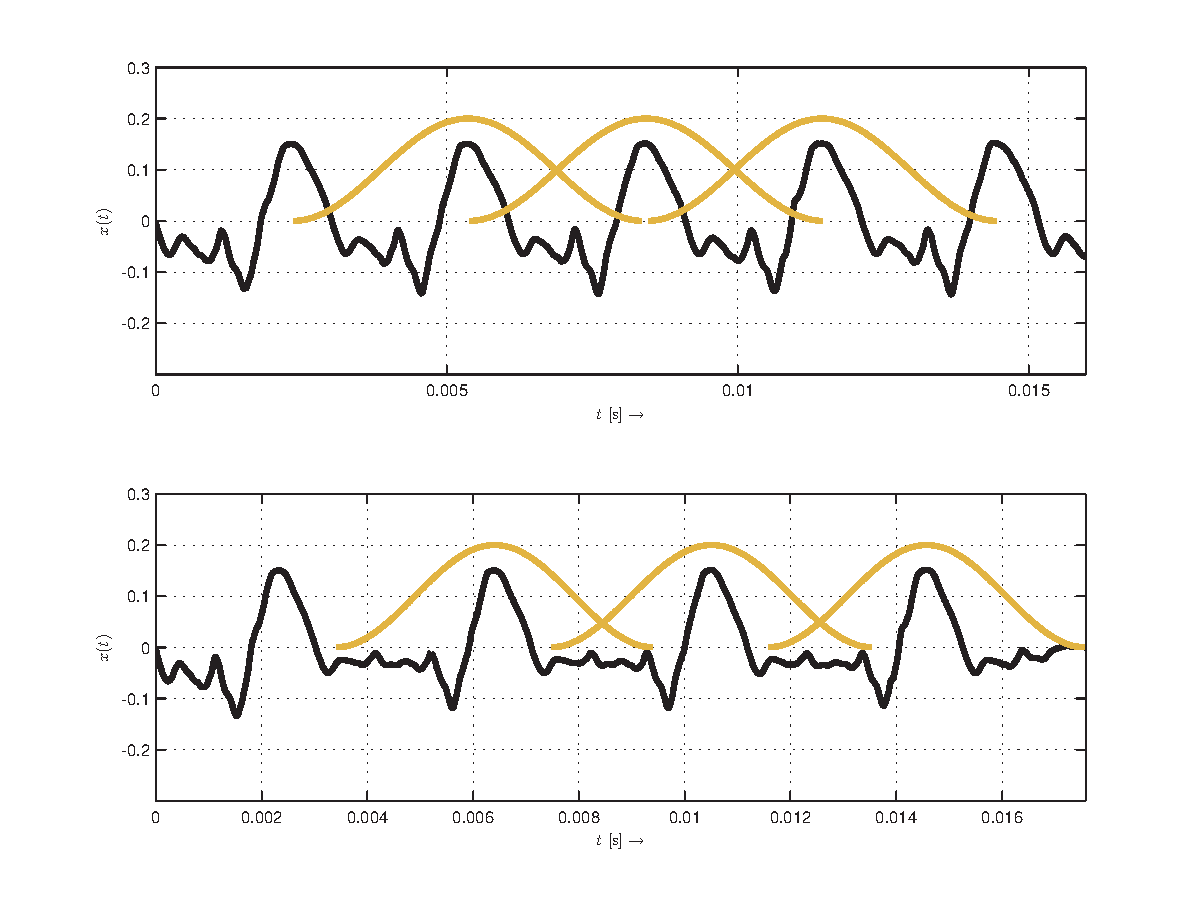
\includegraphics[scale=.25]{graph/PsolaPitch}
                    \end{flushright}   
                    }
        \end{frame}
        \begin{frame}{pitch shifting}{formant preservation: frequency domain}
           \begin{columns}
                \column{.5\textwidth}
                    \begin{itemize}
                        \item \textbf{idea}
                            \begin{itemize}
                                \item   preserve spectral envelope
                            \end{itemize}
                        \bigskip
                        \pause
                        \item \textbf{approach}
                            \begin{enumerate}
                                \item   measure spectral envelope
                                \item   apply inverse envelope (whitening)
                                \item   pitch shift
                                \item   apply spectral envelope
                            \end{enumerate}
                  \end{itemize}
                \column{.5\textwidth}
        \visible<3->{
                    \begin{figure}
                        \centering
                        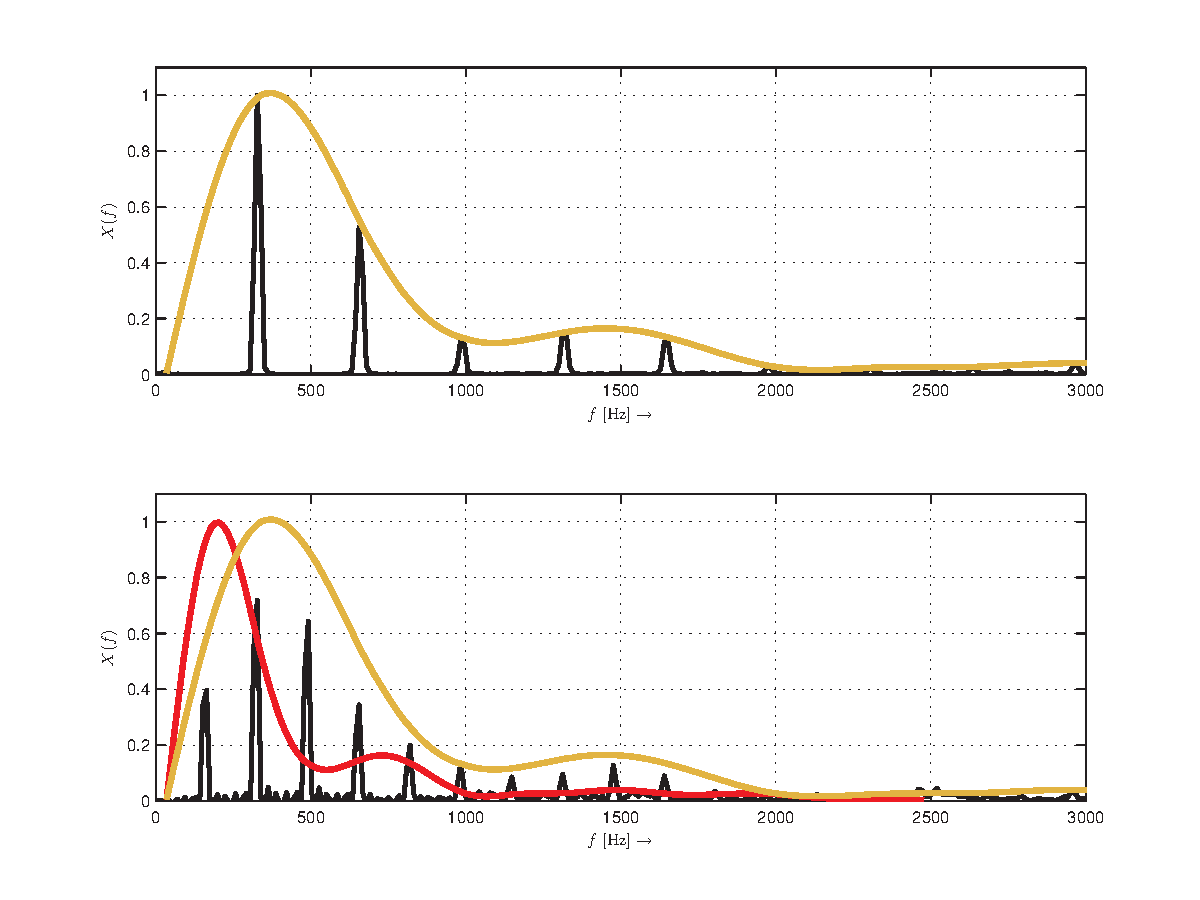
\includegraphics[scale=.25]{graph/SpectralEnvelope}
                    \end{figure}   
                }
            \end{columns}
        \end{frame}
        \begin{frame}{pitch shifting}{spectral envelope estimate}
            \begin{itemize}
                \item   \textbf{approaches}
                    \begin{itemize}
                        \item   LPC coefficients
                        \item   spectral maxima
                    \end{itemize}
                \pause
                \bigskip
                \item   \textbf{potential issues}
                    \begin{itemize}
                        \item   \textit{polyphonic input} audio:\\ 'superposition' of envelopes
                        \item   \textit{very high/low pitch factors}: high frequency boost/cut
                        \item   \textit{estimate resolution}
                            \begin{itemize}
                                \item   too coarse $\rightarrow$ loss of timbre characteristics
                                \item   too fine $\rightarrow$ impress pitch characteristics (harmonic pattern) on spectrum
                            \end{itemize}
                    \end{itemize}
            \end{itemize}
        \end{frame}
        \begin{frame}{pitch shifting}{audio examples}
		\begin{table}
			\begin{center}
				\begin{tabular}{lccc}
                 & OLA & PSOLA & PVOC \\\hline
                orig & \includeaudio{cathy}  &
                     \includeaudio{cathy} &
                     \includeaudio{cathy} \\

                resample $p=\nicefrac{4}{3}$ &\includeaudio{cathyOLApitch}  &
                     \includeaudio{cathySOLpitch} &
                     \includeaudio{cathyPropitch} \\
                formant $p=\nicefrac{4}{3}$&\includeaudio{cathyOLApitchf}  &
                     \includeaudio{cathySOLpitchf} &
                     \includeaudio{cathyPropitchf} 
				\end{tabular}  
			\end{center}
		\end{table}      
                \end{frame}
	
\section{summary}
		\begin{frame}{summary}{time stretching and pitch shifting}
            \begin{itemize}
                \item   pitch stretching and pitch shifting are largely equivalent algorithms
                    \begin{itemize}
                        \item   same artifacts
                        \item   same workload
                    \end{itemize}
                \bigskip
                \item   monophonic time-stretching with PSOLA-based approaches is
                    \begin{itemize}
                        \item   easier to solve
                        \item   has very bad artifacts is pitch tracker is off
                    \end{itemize}
                \bigskip
                \item   polyphonic time-stretching with PV-based approaches is
                    \begin{itemize}
                        \item   complicated due to tradeoffs (e.g., frequency vs time resolution)
                    \end{itemize}
                \bigskip
                \item   general challenges: 
                    \begin{itemize}
                        \item   noisy and transient signals
                        \item   resulting timbre changes
                        \item   perceived naturalness of result
                        \item   time resolution/accuracy due to blocked processing
                    \end{itemize}
            \end{itemize}
 		\end{frame}

\end{document}

